\documentclass{article}
\usepackage[utf8]{inputenc}
\usepackage[spanish]{babel}
\usepackage{amsthm}
\usepackage{amsmath}
\usepackage{amssymb}
\usepackage{graphicx}
\usepackage{wrapfig}
\usepackage[letterpaper, top=0.78in, bottom=0.78in, left=0.98in, right=0.98in]{geometry}
\usepackage[hidelinks]{hyperref}
\usepackage{url}
\usepackage{soul}
\usepackage{tabularx}
\usepackage{csquotes}
\usepackage{enumitem}

\decimalpoint
\renewcommand{\baselinestretch}{1.5}

\begin{document}
    \begin{titlepage}
        \begin{center}
            % School logo
            \begin{figure}
                \centering
                
\includegraphics[scale=0.13]{/home/mona/Pictures/logo_itesm.png}\\ % Logo de la institución
            \end{figure}
            \vspace{5cm}
            % School data
            \LARGE{Instituto Tecnológico y de Estudios Superiores de Monterrey}\\
            \vspace{1cm}
            \large Escuela de Ingeniería y Ciencias \\
            \vspace{0.2cm}
            \large Ingeniería en Ciencias de Datos y Matemáticas \\
            \vspace{0.2cm}
            \large Uso de álgebras modernas para seguridad y criptografía \\
            \vspace{1cm}
            \textbf{Implementación de criptografía de clave pública para protección de comunicaciones con IoT en entornos de monitoreo y consumo de energía.}\\ % Nombre de la tarea
            \vspace{0.7cm}
            % Tabla de integrantes del equipo
            \begin{table}[h!]
                \centering
                \begin{tabular}{ ||c|c|| }
                    \hline
                    Nombre & Matrícula \\
                    \hline
                    Juan Pablo Echeagaray González & A00830646 \\
                    \hline
                    Ricardo Camacho Castillo & A01654132 \\
                    \hline
                    Michelle Yareni Morales Ramón & A01552627 \\
                    \hline
                    Emily Rebeca Méndez Cruz & A00830768 \\
                    \hline
                    Daniela García Coindreau & A00830236 \\
                    \hline
                    Carolina Longoria Lozano & A01721279 \\
                    \hline
                \end{tabular}
            \end{table}
            \vspace{0.7cm}
            \large 	Dr. Alberto F. Martínez \\ % Nombre del profesor 1
            \vspace{0.2cm}
            \large 	Dr. Daniel Otero Fadul\\ % Nombre del profesor 2
            \vspace{0.2cm}
            \large Socio Formador: COCOA, LICORE \\
            \vspace{0.2cm}
            \large Monterrey, Nuevo León \\
            \vspace{0.2cm}
            \large 17 de marzo del 2023 \\
            \vspace{1cm}
        \end{center}
    \end{titlepage}
    % \maketitle

    \tableofcontents
    \listoffigures
    \listoftables
    \clearpage
    \renewcommand{\tablename}{Tabla}

    \section{Introducción}

        Mientras avanzamos en el camino de la industrialización, los datos se vuelven más y más vitales para el funcionamiento de cualquier empresa. Más allá de ser de suma importancia para el análisis de su rendimiento, muchas veces fungen como materia prima de sus procesos. Las fugas de información no son necesariamente nuevas, pero la era digital ha permitido que ocurran de una manera masiva, y ha llegado a afectar a empresas renombradas como Yahoo, Microsoft y Facebook \cite{data_breach_biggest}. Muchas veces estas empresas manejan datos sensibles, y una filtración de datos es un problema grave para ellos y sus usuarios.

        Este es el caso para nuestros socios formadores, \textit{Cocoa} y \textit{LiCore}. \textit{Cocoa} se enfoca en facilitar la transición energías limpias utilizando herramientas digitales \cite{cocoa}, y  \textit{LiCore} se enfoca en desarrollar tecnología electrónica en áreas relacionadas a la energía sostenible. Una parte clave en su proceso consiste en documentar información de la cantidad y calidad de la energía, que al obtenerse pasa a un auditor, y del auditor a un centro de control. Estos datos al ser de carácter sensible, necesitan ser transmitidos por un medio seguro, por lo que es imperativo la implementación de un medio de transporte seguro que se adapte a los dispositivos que utiliza el Socio Formador.

        A continuación estableceremos el objeto de nuestro estudio, plantearemos el problema a ser solucionado y elaboraremos una justificación. Después, haremos una investigación extensa sobre el estado del arte. Analizaremos los recursos disponibles para la resolución del problema, y nuestros objetivos para solucionarlo. Determinaremos la arquitectura de red a ser utilizada y propondremos nuestra metodología. Finalmente, discutiremos los resultados obtenidos.

    % Descripción general de canvas
    \section{Objeto de estudio}

        El caso de estudio general que compete a un proyecto como el presentado es la implementación de un protocolo de clave pública para un \textit{SmartGrid}, que es equivalente a una red heterogénea de dispositivos IoT \cite{smart_grid_def}.

        La implementación de dicha arquitectura viene de la mano con un conjunto de desafíos asociados al poder computacional restringido de los dispositivos IoT, la necesidad de que la comunicación entre los miembros de la red suceda casi en tiempo real, en la disponibilidad de recursos económicos para la construcción y selección de los dispositivos físicos y/o servicios a contratar, y en la técnica a implementar para resguardar los datos de los auditores en una base de datos segura.

        Los datos a enviar serán de carácter energético, conteniendo información del consumo y generación de energía eléctrica asociados a un domicilio y a una etiqueta de tiempo. Los datos generados son de carácter sensible, pues algún agente malicioso podría utilizar algún método de \textit{spyware} para recolectar dichos datos, realizar algún proceso de caracterización para lanzar un ataque acotado y personalizado a los entes asociados al conjunto de datos vulnerados.

    \section{Planteamiento del problema}

        \subsection{Descripción general de la problemática}

            En la Figura \ref{fig:dataExchange} se muestra un esquema simplificado más general de la red \textit{SmartGrid} que se busca asegurar. En primera instancia, se busca proteger el intercambio de información entre cada auditor y el control center. Se busca asegurar la confidencialidad, integridad y autenticidad en todo el proceso de comunicación para que solamente los dispositivos autorizados por el centro deo control puedan publicar y acceder a los datos medidos, que la información medida no sufra de alteración alguna y que existan los medios suficientes para aplicar un criterio de no repudio a los auditores participantes de la red.

            En conjunto con la Figura \ref{fig:dataExchange}, se proporciona la Tabla \ref{tab:component_basic} en la que se enumera y describen las labores de los componentes básicos de la red solicitada por el Socio Formador.
            \begin{table}[htbp]
                \centering
                \begin{tabularx}{\textwidth}{ |l|X|X| }
                    \hline
                    Componente & Función & Dispositivo \\
                    \hline
                    SmartMeter	& Monitoreo de parámetros de consumo y generación de energía eléctrica, envío de datos medidos a su auditor respectivo por medio de WiFi & No aplica \\
                    \hline
                    Auditor	& Recolección de datos de SmartMeters, envío de datos al centro de control & Microcontroladores, tarjetas tipo Raspberry Pi \\
                    \hline
                    Centro de control & Procesamiento de lecturas enviadas por auditores, respaldo encriptado de mediciones en una base de datos & Servidor en la nube \\
                    \hline
                \end{tabularx}
                \label{tab:component_basic}
                \caption{Listado general de los componentes de la red}
            \end{table}

            \begin{figure}[htbp]
                \centering
                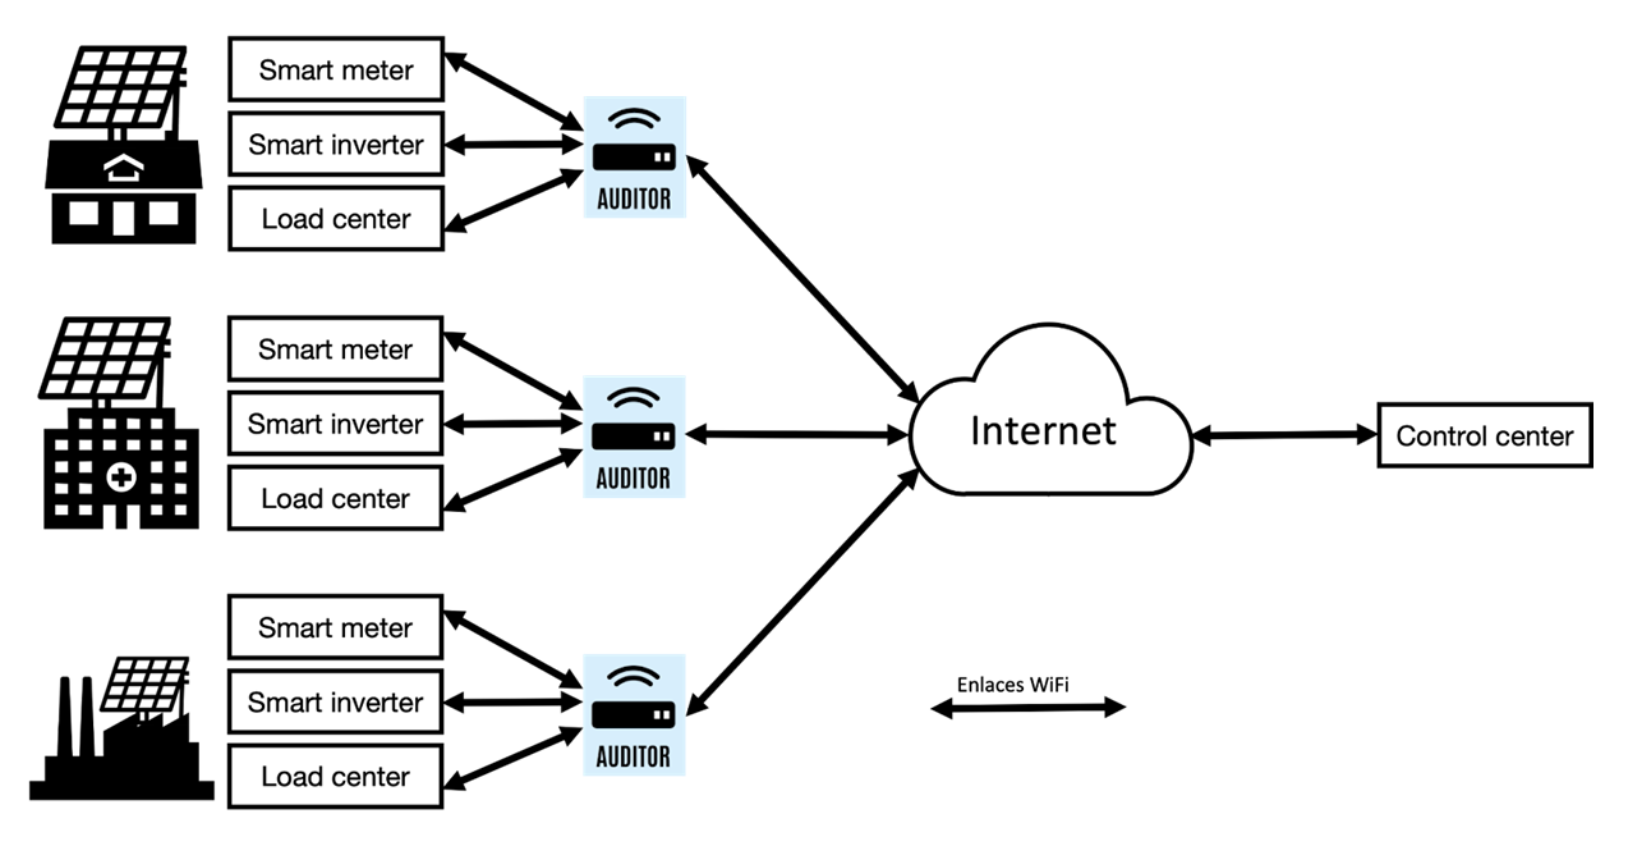
\includegraphics[scale=0.30]{img/dataExchange.png}
                \caption{Intercambio de Datos a ser Protegido [Extraído de CANVAS]}
                \label{fig:dataExchange}
            \end{figure}

        \subsection{Delimitación del problema}

            Para fines académicos a organización socio-formadora propone el escenario representado en la Figura \ref{fig:esquema}. Se dispondrá de dos auditores, que reportan el consumo y generación de energía eléctrica de 2 residencias distintas. Los datos en cuestión no serán obtenidos en tiempo real, sino que han sido proporcionados por el socio-formador en el formato de un archivo csv con los registros históricos de las mediciones.

            Los datos recolectados por los auditores deben de ser enviados por internet protegidos hasta que lleguen al Centro de Control. En el Centro de Control, los datos serán almacenados en una base de datos en donde serán respaldados con un esquema de encriptado seguro.

            \begin{figure}[h]
                \centering
                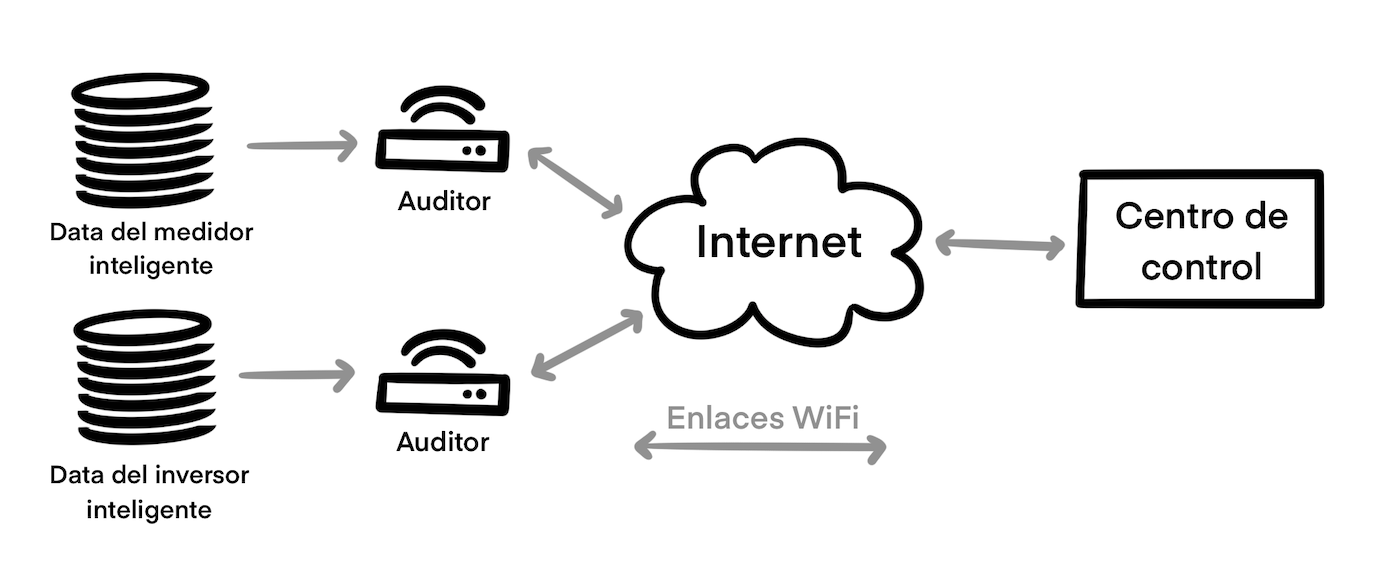
\includegraphics[scale=0.35]{img/esquema_reto.png}\\
                \caption{Esquema sugerido para la prueba de concepto (PdC).[Imagen referenciada de CANVAS]}
                \label{fig:esquema}
            \end{figure}

    \section{Justificación}

        \subsection{Enfoque en Sostenibilidad}

            Nuestro propósito se alinea con múltiples de los Objetivos de Desarrollo Sustentable de las ONU.
            \begin{itemize}
                \item \textbf{Objetivo 9}: \enquote{Construir infraestructuras resilientes, promover la industrialización sostenible y fomentar la innovación.}  \cite{obj9} Lo vemos reflejado en nuestro deseo de innovar e industrializar sin sacrificar lo sostenible.
                \item \textbf{Objetivo 11}: \enquote{Lograr que las ciudades sean más inclusivas, seguras, resilientes y sostenibles.} \cite{obj11} Este objetivo esta integrado en las bases del proyecto, con la intención del socio formador de acercar la energía al consumidor, y con su elección de utilizar energías renovables.
                \item \textbf{Objetivo 12}: \enquote{Garantizar modalidades de consumo y producción sostenibles.}\cite{obj12} Es uno de nuestros principales enfoques, al utilizar algoritmos ligeros que serán lo mas sostenibles posibles, y al ayudar a que un proceso de producción de energía sostenible pueda efectuar de manera segura.
            \end{itemize}

        \subsection{Dimensión legal y económica}

            De acuerdo a IBM, el costo global promedio en 2022 de una filtración de datos fue de 4 millones de dólares \cite{cost_DB}. Esta cifra sigue un patrón de aumento a través del tiempo, lo que nos indica que cada vez se vuelve más caro tener datos desprotegidos. Lo económico no es lo único que se ve afectado por un ataque de esta naturaleza. El estudio del Instituto Ponmeon, "The Aftermath of a Mega Data Breach: Consumer Sentiment", clasifica a las filtraciones de datos como el tercer factor más influyente para la reputación de una empresa, junto con desastres naturales y mal servicio al cliente \cite{ponmeon}.

            Cada segundo se conectan a internet alrededor de 127 dispositivos nuevos. Estos dispositivos atraen a ciberdelicuentes debido a que muchas de las personas que compran dichos aparatos desconocen los puntos importantes de ciberseguridad al momento de adquirirlo, el cual puede poner en riesgo la privacidad del usuario. Los dispositivos IoT usualmente son objetivo de ataques forzados. Los ataques forzados usando motores de búsqueda especializados en donde se seleccionan equipos de protocolos disponibles para conexión, así forzando de manera automática los nombres de usuario y contraseñas comunes. Se estima que a nivel global, la cifra de ataques a dispositivos IoT es mayor a los mil 500 millones. En México, el primer semestre de 2021 se detectaron 661 mil 715 ataques a dispositivos IoT \cite{rios_2022}. La cantidad de ataques tuvo un incremento de 197 por ciento a comparación con el año 2020 en donde se registran 222 mil 599.

            Como se ha mencionado anteriormente los ataques a dispositivos IoT son comunes y costosos, a continuación se describirán algunos ataques o vulnerabilidades encontradas en dispositivos por el mal uso de primitivas criptográficas:

            \begin{itemize}
                \item En noviembre 2016, cibercriminales apagaron la calefacción de dos edificios en la ciudad finlandesa de Lappeenranta. Después de este ataque, se lanzó un segundo ataque DDoS, en donde obligaron a los controladores de calefacción a reiniciar el sistema repetidamente así evitando que la calefacción se encendiera. Este fue un ataque severo ya que en Finlandia se experimentan temperaturas muy bajas en esa época del año \cite{husar_2022}.
                \item En el 2016, investigadores encontraron que alrededor de 100 millones de vehículos Volkswagen vendidos desde 1995 pueden ser atacados por cibercriminales con una facilidad relativa para abrir puertas de forma inalámbrica sin tener la llave. Los vehículos eran vulnerable debido a que se usaron una mínima cantidad de claves privadas compartidas, en donde una vez que se viole una sola clave privada entonces millones de vehículos se verán comprometidos ya que los 100 millones de vehículos y sus llaveros fueron programados con pocas claves secretas comunes utilizadas en todo el mundo. Esto comprometía la seguridad de los pasajeros ya que ellos suponen que el vehículo esta bien cerrado comprometiéndolos a un robo en la carretera, a que criminales coloquen discretamente un objeto o una persona con intenciones maliciosas dentro del automóvil, pone en riesgo la computadora de a bordo del vehículo en donde el criminal puede  desactivar los frenos mientras se enciende el sistema de limpiaparabrisas en una curva, etc  \cite{garcia_oswald_kasper_pavlides}.
                \item En el 2017, se descubrió que decenas de millones de dispositivos como cámaras de vigilancia de aeropuertos, sensores, equipos de red y dispositivos de IoT eran vulnerables debido a una falla que permitía a los cibercriminales obtener control remoto sobre los dispositivos o bloquearlos. La vulnerabilidad encontrada la nombraron "Devil's Ivy". Esta fue descubierto debido a que investigadores de Senrio quienes seleccionaron cámaras de seguridad de alta gama fabricadas por Axis Communications en donde 249 de los 251 cámaras eran vulnerables a atacantes remotos no autenticados que podían interpretar una transmisión de vídeo, reiniciar cámaras o pausar una transmisión de vídeo mientras cometen un delito \cite{spring_2019}. Encontraron que no solamente Axis Communications usaba este software defectuoso si no que otras 34 compañías como Microsoft, IBM, Xerox y Adobe.
            \end{itemize}

    \section{Estado del arte} \label{sec:state_art}

        La interconexión de dispositivos IoT al internet es uno de los principales desafíos a los que se enfrentan los ingenieros de esta era digital. La naturaleza de recursos restringidos de los dispositivos disponibles vuelve complicada la aplicación directa de los algoritmos y protocolos criptográficos usuales que pueden correr sin más inconveniente en un ordenador de uso personal o un teléfono inteligente.

        Esta dificultad ha motivado el diseño de esquemas criptográficos ligeros que ofrecen un balance entre la robustez y seguridad de las interconexiones para con el costo y consumo energético en el que incurren los dispositivos.

        \subsection{Dispositivos IoT Endpoint}

            El análisis inicial parte de la selección óptima del dispositivo que fungirá como auditor en la problemática propuesta, la literatura moderna se enfoca en microcontroladores o tarjetas que no suelen sobrepasar el costo de 50 USD. En \cite{el2018analysis} se realiza un sumario general de las tarjetas usadas comúnmente para después concretar un enfoque del desempeño de distintos algoritmos en una tarjeta \textit{Raspberry Pi 3B}.

            Una alternativa atractiva a una tarjeta de gama superior como la anterior, es el microcontrolador \textit{ESP32}. En \cite{anand2019secure} se emplea dicho microcontrolador en un ambiente similar a la problemática planteada por las bondades de la tarjeta que incluye una suite acelerada para la generación de claves públicas y privadas con RSA, la firma con SHA-256 y la facilidad de generar números suficientemente aleatorios (en el contexto criptográfico).

            De forma similar se propone considerar la tarjeta \textit{Raspberry Pi Pico}; no se ha encontrado un artículo científico en el que se detalle su uso en un entorno como el propuesto, pero se recalca que las especificaciones técnicas de la tarjeta descritas en \cite{pico_specs} son equivalentes a las del \textit{ESP32}.

            \begin{table}[htbp]
                \centering
                \begin{tabularx}{\textwidth}{ |X|X|l|X|X|X|X|X| }
                    \hline
                    Nombre & Chip & RAM & Disco Duro & Conectividad & OS & Lenguaje & Referencia \\
                    \hline
                    Raspberry Pi Model 3 B & ARM Cortex A53 & 1 GB & SD card & WiFi, Ethernet  & Raspbian OS & Python, C++, etc...  & \cite{el2018analysis}   \\
                    \hline
                    ESP32 & Tensilica Xtensa LX6 & 320 kB & 448 KB Rom & WiFi, Bluetooth & - & Micropython, Circuit Python & \cite{anand2019secure} \\
                    \hline
                    Raspberry Pi Pico & Arm Cortex-M0+ & 264 kB & 2 MB & WiFi & - & Micropython, C, C++ & \cite{pico_specs} \\
                    \hline
                \end{tabularx}
                \label{tab:controllers}
                \caption{Listado de microcontroladores factibles}
            \end{table}

        \subsection{Encriptado asimétrico}

            La parte más complicada de la comunicación segura entre dispositivos IoT ocurre en la generación, firmado y verificación de mensajes utilizando clave pública y privada. En la actualidad existen 3 principales métodos de encriptado de clave pública que se utilizan entornos IoT como el nuestro, de forma particular se suele analizar el desempeño de RSA, DSA y ECDSA.

            En \cite{el2018analysis} se realiza una comparativa de estos 3 algoritmos en una tarjeta Raspberry Pi 3B. El estudio encontró que en promedio a RSA le toma 20 veces más tiempo firmar un mensaje que ECDSA y utiliza un tamaño de llave 16 veces superior para el mismo nivel de seguridad; el único rubro en el que RSA supera a ECDSA es en el verificado de mensajes, donde es 3 veces más rápido. Se puede ver que en promedio ECDSA tiene el mejor desempeño.

        \subsection{Encriptado simétrico}

            Una vez que se ha establecido un secreto en común entre 2 entes se puede aplicar alguna de las técnicas de encriptado simétrico que conocemos; esta suele ser una de las partes más sencillas de cualquier protocolo criptográfico ya que suele ser computacionalmente eficiente y rápido de calcular para evitar problemas de latencia en los procesos de comunicación.

            En \cite{el2018analysis} se realizó una comparativa de los algoritmos de cifrado DES, 3DES, AES128, AES192 y AES256. Una conclusión esperada era que los algoritmos de la clase DES tuvieran una huella reducida a comparación de la suite de AES; a pesar de que su estudio confirma el supuesto, el NIST tiene registros de vulnerabilidades de este algoritmo desde el 2016 \cite{des_vulnerable}.
        \subsection{Firma digital}

            Una parte fundamental de los algoritmos de encriptado descritos es la función \textit{hash}. La principal aportación de este componente es que brinda la habilidad de que un destinatario se asegure de que el mensaje que haya recibido no ha sido modificado en el transcurso de su envío.

            Algunas de las cualidades que deben tener estas funciones hash es la sencillez con la que puede ser computada y el que sea segura a colisiones; se entiende por colisión el evento en el que a dos objetos distintos se les asigna un mismo hash.

            En \cite{el2018analysis} se realiza un análisis general del desempeño de las funciones hash MD5, SHA-1, SHA-256 y SHA-512 en una tarjeta Raspberry Pi 3B. La investigación encuentra que las funciones hash MD5 y SHA-1 son las más veloces del conjunto original, sin embargo se ha declarado desde el 2008 que MD5 no es una función hash segura \cite{md5_vulnerable}; para el caso de SHA-1 ya se ha emitido un comunicado del \textit{NIST} que recomienda dejar de utilizar esta función \cite{sha1_vulnerable}.

            En \cite{rao2019comparative} se realiza un estudio similar al anterior, pero enfocado a la función hash necesaria para el firmado con curvas elípticas. Su conjunto de pruebas consistió en parte de las mismas funciones anteriores en añadidura de HAVAL, KECCAK, y BLAKE. El estudio encontró que la familia SHA es de las mejores disponibles, pero es sobrepasada por la función hash BLAKE en cuanto a uso en curvas elípticas concierne.

        \subsection{Protocolos criptográficos}

            Al final del día las funciones y componentes mencionadas representan partes estrictamente aisladas del protocolo criptográfico a implementar para asegurar las conexiones en la red propuesta. Es por eso que después se proponen mezclas y técnicas que implementan los algoritmos criptográficos base que después son acotados y personalizados a diferentes casos de estudio.

            En \cite{abreu2020identity} se propone un enfoque similar a arquitecturas cliente-servidor, en el que se envían datos por medio de HTTPS haciendo uso de TLS para asegurar las vías de comunicación. El estudio propuso una arquitectura que necesita de menos mensajes para asegurar un canal de comunicación, pero que no logra concretar una política de acceso detallada basada en los recursos a los cuales se desea acceder y/o modificar.

            En \cite{lohachab2019ecc} se propone un esquema ligero que no utiliza el concepto de certificados para el proceso de autenticación y autorización, para ser remplazados por un esquema de comunicación sobre MQTT incluyendo \textit{hasheo} con firmado de claves públicas generadas de forma local, sin que se incurra en un alto consumo energético o que se añada una latencia descomunal al proceso de comunicación.

    \section{Recursos disponibles}

        La organización socio formadora ha estipulado que el auditor propuesto no puede superar un costo total de 100 USD; sin embargo ha manifestado su preferencia por un auditor que tenga un costo alrededor de los 50 USD. Para emular dichos dispositivos se propone el uso de dos tarjetas de microprocesador Raspberry Pi 3B
        (modelo a determinar en base a disponibilidad del laboratorio de robótica).

        Para la emulación del centro de control se propone utilizar una instancia de EC2 de Amazon Web Services, en la que se emulará un servidor con una base de datos que utilice MySQL.

    \section{Objetivos}

        Los objetivos de este proyecto deben de ser vistos desde 2 esquemas cualitativos:
        \begin{enumerate}
            \item \textbf{Fines académicos}: Desarrollo de una primitiva criptográfica de clave pública sin hacer uso de bibliotecas de terceros para el cómputo de las claves. Aclarando que no existen limitaciones para el uso de bibliotecas que realicen de forma eficiente algunas operaciones matemáticas necesarias
            \item \textbf{Términos ingenieriles}: Desarrollo de una arquitectura de red que permita que un conjunto de dispositivos auditores envíen lecturas de consumo y generación de energía eléctrica a un centro de control por medio de una conexión WiFi. Se parte de que los auditores tienen poder computacional bajo, y los datos generados deben de ser enviados y almacenados de forma segura.
        \end{enumerate}

        En términos cuantitativos se plantean las siguientes metas:
        \begin{enumerate}
            \item Costo total del dispositivo auditor menor a \textbf{100 USD} por pieza.
            \item El tiempo de envío seguro de datos debe de ser menor a \textbf{15 minutos}, puesto que las lecturas son generadas en ventanas de tiempo de 15 minutos.
        \end{enumerate}

    \section{Arquitectura de red propuesta}

        Hablar más a detalle de la arquitectura propuesta, enunciando qué componente fungirá cada papel, es como lo que el profe dice de "ponerle nombre y apellido", proponer una nomenclatura para generar identificadores únicos?

        % Seguir arquitectura propuesta por el paper de ECC

        % Imagen de diagrama de red propuesto

        \begin{figure}[htbp]
            \centering
            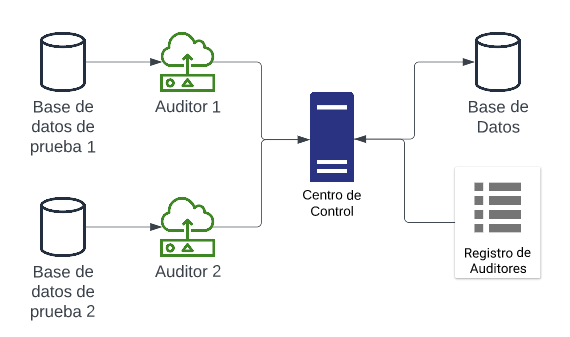
\includegraphics[scale=0.5]{img/arquitectura_propuesta.png}
            \label{fig:proposed_architecture}
            \caption{Esquema de arquitectura propuesta}
        \end{figure}

        \subsection{Sumario de componentes}

            \begin{table}[htbp]
                \centering
                % \setlength{\leftmargini}{0.4cm}
                \scalebox{0.7}{
                \begin{tabular}{| m{2cm} | m{3cm} | m{5cm} | m{9cm} |}
                    \hline
                    Nombre & Manufactura & Arranque & Producción \\
                    \hline
                    % -------------------------------------------------
                    Auditor 1 / Raspberry Pi 3B &
                    \begin{itemize}[noitemsep]
                        \item Carga de función hash
                        \item Contraseña pseudo-aleatoria
                        \item Parámetro secreto $s$
                        \item Instalación de software base
                    \end{itemize} &
                    \begin{itemize}[noitemsep]
                        \item Registro de Smart Meters (esquema similar) *
                        \item Generación de datagrama de identificación
                        \item Envío de datos de identificación a Centro de Control
                    \end{itemize} &
                    \begin{itemize}[noitemsep]
                        \item Recepción de datos de Smart Meters (lectura de datos de prueba)
                        \item Encriptado con curva elíptica del datagrama del SmartMeter
                        \item Pseudo-firma con función hash escogida por Centro de Control
                    \end{itemize} \\
                    \hline
                    % -------------------------------------------------
                    Auditor 2 / Raspberry Pi 3B &
                    \begin{itemize}[noitemsep]
                        \item Carga de función hash
                        \item Contraseña pseudo-aleatoria
                        \item Parámetro secreto $s$
                        \item Instalación de software base
                    \end{itemize} &
                    \begin{itemize}[noitemsep]
                        \item Registro de Smart Meters (esquema similar) *
                        \item Generación de datagrama de identificación
                        \item Envío de datos de identificación a Centro de Control
                    \end{itemize} &
                    \begin{itemize}[noitemsep]
                        \item Recepción de datos de Smart Meters (lectura de datos de prueba)
                        \item Encriptado con curva elíptica del datagrama del SmartMeter
                        \item Pseudo-firma con función hash escogida por Centro de Control
                    \end{itemize} \\
                    \hline
                    % -------------------------------------------------
                    Centro de Control / EC2 Server &
                    Adquisición de instancia de EC2 &
                    \begin{itemize}[noitemsep]
                        \item Selección de parámetros de curva elíptica
                        \item Selección de función hash segura contra colisiones
                        \item Asignación de hash de identidad para cada auditor
                    \end{itemize} &
                    \begin{itemize}[noitemsep]
                        \item Recepción a los datos publicados por el auditor
                        \item Autenticación de la identidad del auditor
                        \item Desencriptado y preprocesamiento del datagrama recibido
                        \item Envío de actualizaciones de software al auditor para CI/CD
                        \item Validación física de los datos recibidos *
                    \end{itemize} \\
                    \hline
                    % -------------------------------------------------
                    Base de Datos &
                    No aplica &
                    Inicialización de esquema de base de datos (predefinido) &
                    \begin{itemize}[noitemsep]
                        \item Procesado de datos recibidos por el centro de control
                        \item Respaldo de datos en la base de datos
                        \item Encriptado de la base de datos
                    \end{itemize} \\
                    \hline
                    % -------------------------------------------------
                \end{tabular}}
                \label{tab:component_summary}
                \caption{Resumen de componentes empleados}
            \end{table}

    \section{Medio de contacto}\label{sec:contact}

        El desarrollo del proyecto así como la redacción del presente documento es un trabajo conjunto de:
        \begin{itemize}[noitemsep]
            \item Juan Pablo Echeagaray González
            \item Ricardo Camacho Castillo
            \item Michelle Yareni Morales Ramóz
            \item Emily Rebeca Méndez Cruz
            \item Daniela García Coindreau
            \item Carolina Longoria Lozano
        \end{itemize}

        Así mismo se destacan los siguientes profesores, como asesores y supervisores de los avances en el desarrollo del proyecto:
        \begin{itemize}[noitemsep]
            \item Dr. Alberto F. Martínez
            \item Dr. Daniel Otero Fadul
        \end{itemize}

        El benefactor principal del proyecto es la organización \textit{LiCore}, la comunicación con la organización se vio llevada principalmente por el Dr. Iván S. Razo-Zapata.

        En caso de encontrar fallas en el código fuente, o que se necesite de una aclaración de la implementación propuesta; se pide que se abra un \textit{issue} en el repositorio en GitHub que puede ser accedido desde la siguiente \href{https://github.com/JuanEcheagaray75/licore-pki}{liga}.

    \clearpage
    \bibliographystyle{IEEEtran}
    \bibliography{references.bib}

\end{document}
